\documentclass[xcolor=dvipsnames,hyperref={pdfpagelabels=false}]{beamer}

\usetheme{Berkeley}

\let\Tiny=\tiny

\newcommand{\bi}{\begin{itemize}}
\newcommand{\ei}{\end{itemize}}
\newcommand{\be}{\begin{enumerate}}
\newcommand{\ee}{\end{enumerate}}
\newcommand{\I}{\item}
\newcommand{\f}{\frame}
\newcommand{\ft}{\frametitle}

\title{Status of the Offline Software}
\subtitle{GlueX Collaboration Meeting}
\author[M.\ Ito]{Mark M.\ Ito}
\date{May 22, 2012}
\institute[JLab]{Jefferson Lab}

\begin{document}

\f{\titlepage}

\section{Major Topics}

\f{
\ft{Major Topics}
Dedicated talks:
\bi
\I Geant4: Richard
\I Tracking: Simon and Paul M.
\I Calorimetry: Will L.
\I Offline Software Review: David L., special session with review talks
\ei
}

\section{Software Topics}

\frame<1>[label=topics-one]{
\ft{Software Topics 1}

\bi
\I<alert@1> Single-charged-track tests running: Simon
  \bi
  \I every Tuesday and Friday
  \I runs off the nightly build
  \ei
\I<alert@2> Reconstruction Output Format: UConn HDDM
\I<alert@3> Adopted CLHEP as an official GlueX package
  \bi
  \I Used by AmpTools, Geant4, Levenberg-Marquardt track fitting
  \ei
\ei
}

\f{
\ft{Single-track test example (May 18)}
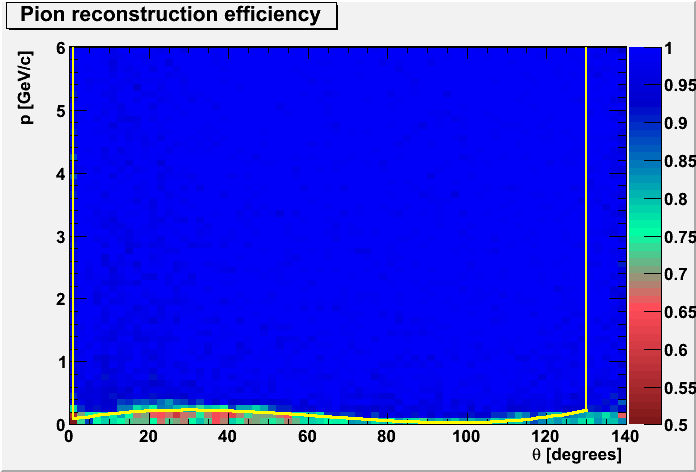
\includegraphics[height=2.8in]{pion_efficiency.png}
}

\f{
\ft{Single-track test example (May 18)}
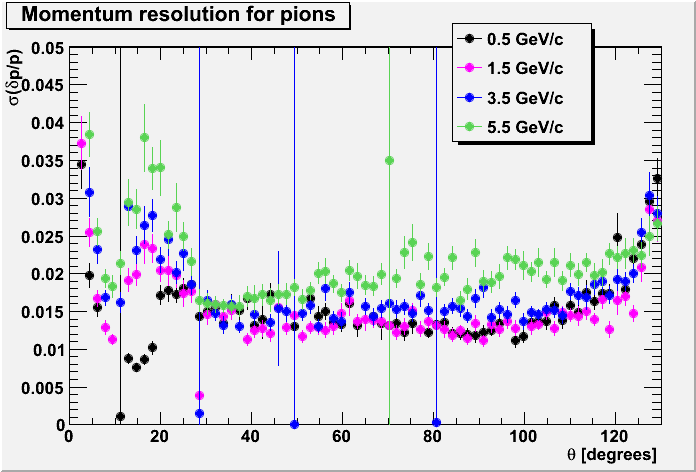
\includegraphics[height=2.8in]{pion_dp_vs_theta.png}
}

\againframe<2-3>{topics-one}

\f{
\ft{Software Topics 2}
\bi
\I EventStore
  \bi
  \I<alert@1> System for disk-resident reconstructed data: from CLEO via Matt
  \I<alert@2> Creating skims without duplication of events themselves by storing only "pointers" to events
  \I<alert@3> Hooks for specifying the version of the code used to reconstruct events
  \I<alert@4> Hooks for skimming events based on various database-resident criteria
  \I<alert@5> Possibility for using alternate reconstruction code to over-ride that used on previously reconstructed data
  \I<alert@6> Feasibility needs studying
  \ei
\ei
}

\f{
\ft{Software Topics 3}
\bi
\I<alert@1> Restructuring of high-level reconstruction classes: Paul M.
\I<alert@2> Secondary vertices now stored in HDGeant output: Beni, Richard
\I<alert@3> Updated documentation on kinematic fitting: Will L.
\I<alert@4> New JANA release, 0.6.4: David
  \bi
  \I  Xerces-c 3.x support
  \ei
\I<alert@5> Rad-hard insert removed from FCAL
\I<alert@6> Issue identified with sampling fluctuations in BCAL simulation: Andrei, Irina
\I<alert@7> Start counter geometry has been updated to 30 sector design: Puneet, Simon
\ei

}

\section{Summary}

\begin{frame}[fragile]
\ft{Summary}
\bi
\I Continuous progress
\I Reconstruction transitioning to next level
\I Lots of projects to be claimed
\I Software review preparation giving offline project overview
\ei
\vfill
\hrule
\tiny
\begin{verbatim}
$Id$
\end{verbatim}

\end{frame}

\end{document}

%%% end of latex file %%%%
